\section{The coherence of light}

\epigraph{Нахрена нам зеркала, на дворе 20 век.}{Петров М. И.}

\subsection{Bunching and antibunching of photons}

Lets consider Michelson stellar interferometer (fig \ref{fig:stellar}). From distant stars the two light beams is coming to our set-up. Light is an electromagnetic wave, so we can write:
\begin{equation}
	\vec{E} = \vec{E}_{\vec{k}} \left( e^{i \vec{k} \vec{r}_{M_1}}  + e^{i \vec{k} \vec{r}_{M_2}} \right) + \vec{E}_{\vec{k}'} \left( e^{i \vec{k'} \vec{r}_{M_1}} + e^{i \vec{k}' \vec{r}_{M_2}} \right).
\end{equation}
If we decide to compute the intensity, we will get { \textcolor{red} {(see Scully)}}
\begin{equation}
	I = \langle \vec{E} \cdot \vec{E}^* \rangle_t  = 4 I_0 \left( 1 + \underbrace{\cos \left[\frac{\left( \vec{k} + \vec{k}' \right) \vec{r}_0}{2}\right]}_{\text{fast term}} \underbrace{\cos \left[{\textcolor{red}\half}  k r_0 \varphi \right]}_{\text{slow term}} \right),
\end{equation}
where $\vec{r}_0 = \vec{r}_{M_1} - \vec{r}_{M_2}$, {\textcolor{red}{$I_0=\langle \vec{E}_{\vec{k}} \cdot \vec{E}_{\vec{k}}^* \rangle_t=\langle \vec{E}_{\vec{k'}} \cdot \vec{E}_{\vec{k'}}^* \rangle_t$}}. To make out light and dark spots we need the following condition
\begin{equation}
	k r_0 \varphi \approx \frac{\pi}{{\textcolor{red} 1}} \qquad \to \qquad \varphi = \frac{\pi}{k r_0}.
\end{equation}
It means that to change light spot to the dark one  we need $\Delta r_0 = \frac{\pi}{k \varphi}$. So the bigger distance between mirrors $M_1$ and $M_2$, the better resolution we get (we will be able to detect smaller $\varphi$). But there appear to be a lot of technical troubles.
\begin{figure}
	\centering
	
\includegraphics[width=0.5\linewidth]{fig/L3/Ij8NUO6Gat0}
	\caption{wow such Jesus}
	\label{fig:jesus}
\end{figure}

One can chose another pill and built a set up with two distant photodetectors (fig \ref{fig:new_stellar}). Now we don't have annoying mirrors and measure only currents $i_1$ and $i_2$, which are proportional to the intensities $I_1$ and $I_2$ of incident light beams. By this framework we can significantly increase $r_0$ and this will lead to a higher resolution. People who did very precise measurements, noticed that they no longer measure intensities of indecent light, but only noises of almost single photons.


\begin{figure}
	\centering
	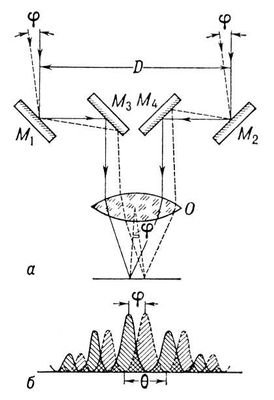
\includegraphics[width=0.6\linewidth]{fig/L3/stellar}
	\caption{A Michelson stellar interferometer}
	\label{fig:stellar}
\end{figure}


\begin{figure}
	\centering
	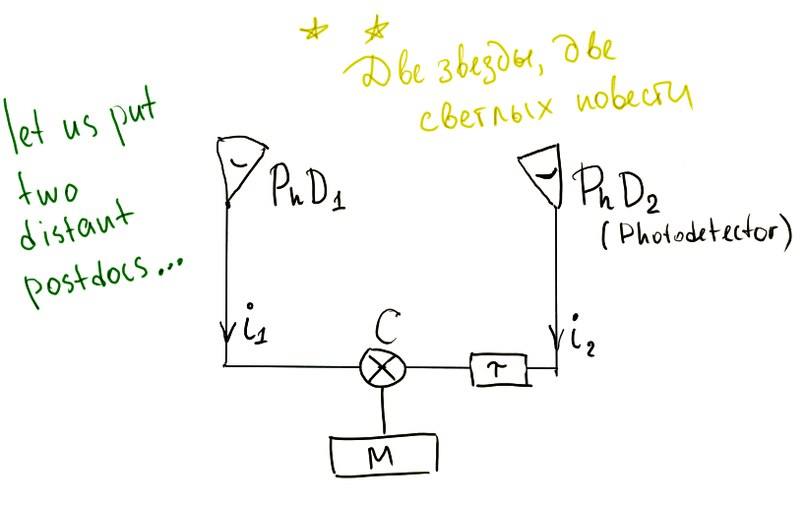
\includegraphics[width=0.5\linewidth]{fig/L3/new_stellar}
	\caption{A symmetric interferometer with distant photodetectors}
	\label{fig:new_stellar}
\end{figure}




Now lets take a look at this situation from a theoretical point of view. Let us compute the following correlator
\begin{equation}
	g^{(2)} = \frac{\langle i_1, i_2 \rangle }{\langle i_1 \rangle \langle i_2 \rangle},
\end{equation}
where
\begin{equation}
	i_1 = \langle i_1 \rangle + \Delta i_1, \qquad i_2 = \langle i_2 \rangle + \Delta i_2, \qquad \langle i_1 \rangle = \langle i_2 \rangle = i_0.
\end{equation}
Then we can write
\begin{equation}
	g^{(2)} = \frac{i_0^2 + \langle \Delta i_1, \Delta i_2 \rangle}{i_0^2} = 1 + \frac{\langle \Delta i_1, \Delta i_2 \rangle}{i_0^2}.
\end{equation}
So in fact one measured the average of $\Delta i_1$ and $\Delta i_2$. To study the issue in more details the so called \textit{HBT experiment} was done. The principle scheme of the set up it shown on fig \ref{fig:HBT_exp}. The heart of the matter is that method allows to avoid the atmospherically sensitive terms (fast terms) like $\cos \left[ \frac{(\vec{k} + \vec{k}') \cdot \vec{r}_0}{2} \right]$.

\begin{figure}
	\centering
	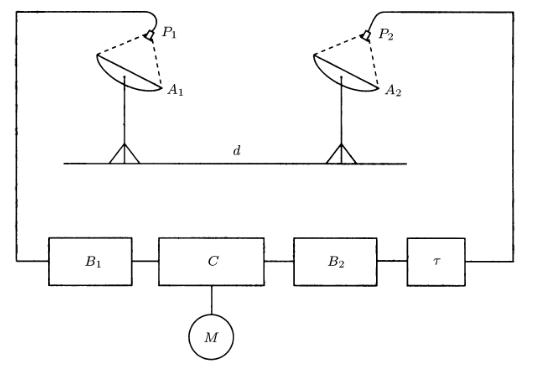
\includegraphics[width=0.6\linewidth]{fig/L3/HBT_exp}
	\caption{Schematic diagram of the Hanbury Brown-Twiss stellar intensity interferometer. Here $P_1$ and $P_2$ are photodetectors, $A_1$ and $A_2$ are the mirrors, $B_1$ and $B_2$ are the amplifiers, $\tau$ is the delay time, $C$ is a multiplier, and $M$ is the integrator}
	\label{fig:HBT_exp}
\end{figure}


